\section{Prototypes}
\label{result:prototypes}
Below is a list of features that members of an experience design core team would prefer to have in the tool in question:
\begin{itemize}
  \item List all features of lo-fi prototype here
  \item More lists
\end{itemize}
\subsection{Lo-Fi}
 Several different sketches and concepts were created to obtain a diversity of interfaces to test. Following concepts and elements where selected for the Hi-fi prototyping phase after tests were conducted on all sketches.

\subsubsection{Main interface - Belt UI}

\subsubsection{UI Selectors}

\subsubsection{Object selection and manipulation}



\begin{figure}
\begin{subfigure}{.5\textwidth}
  \centering
  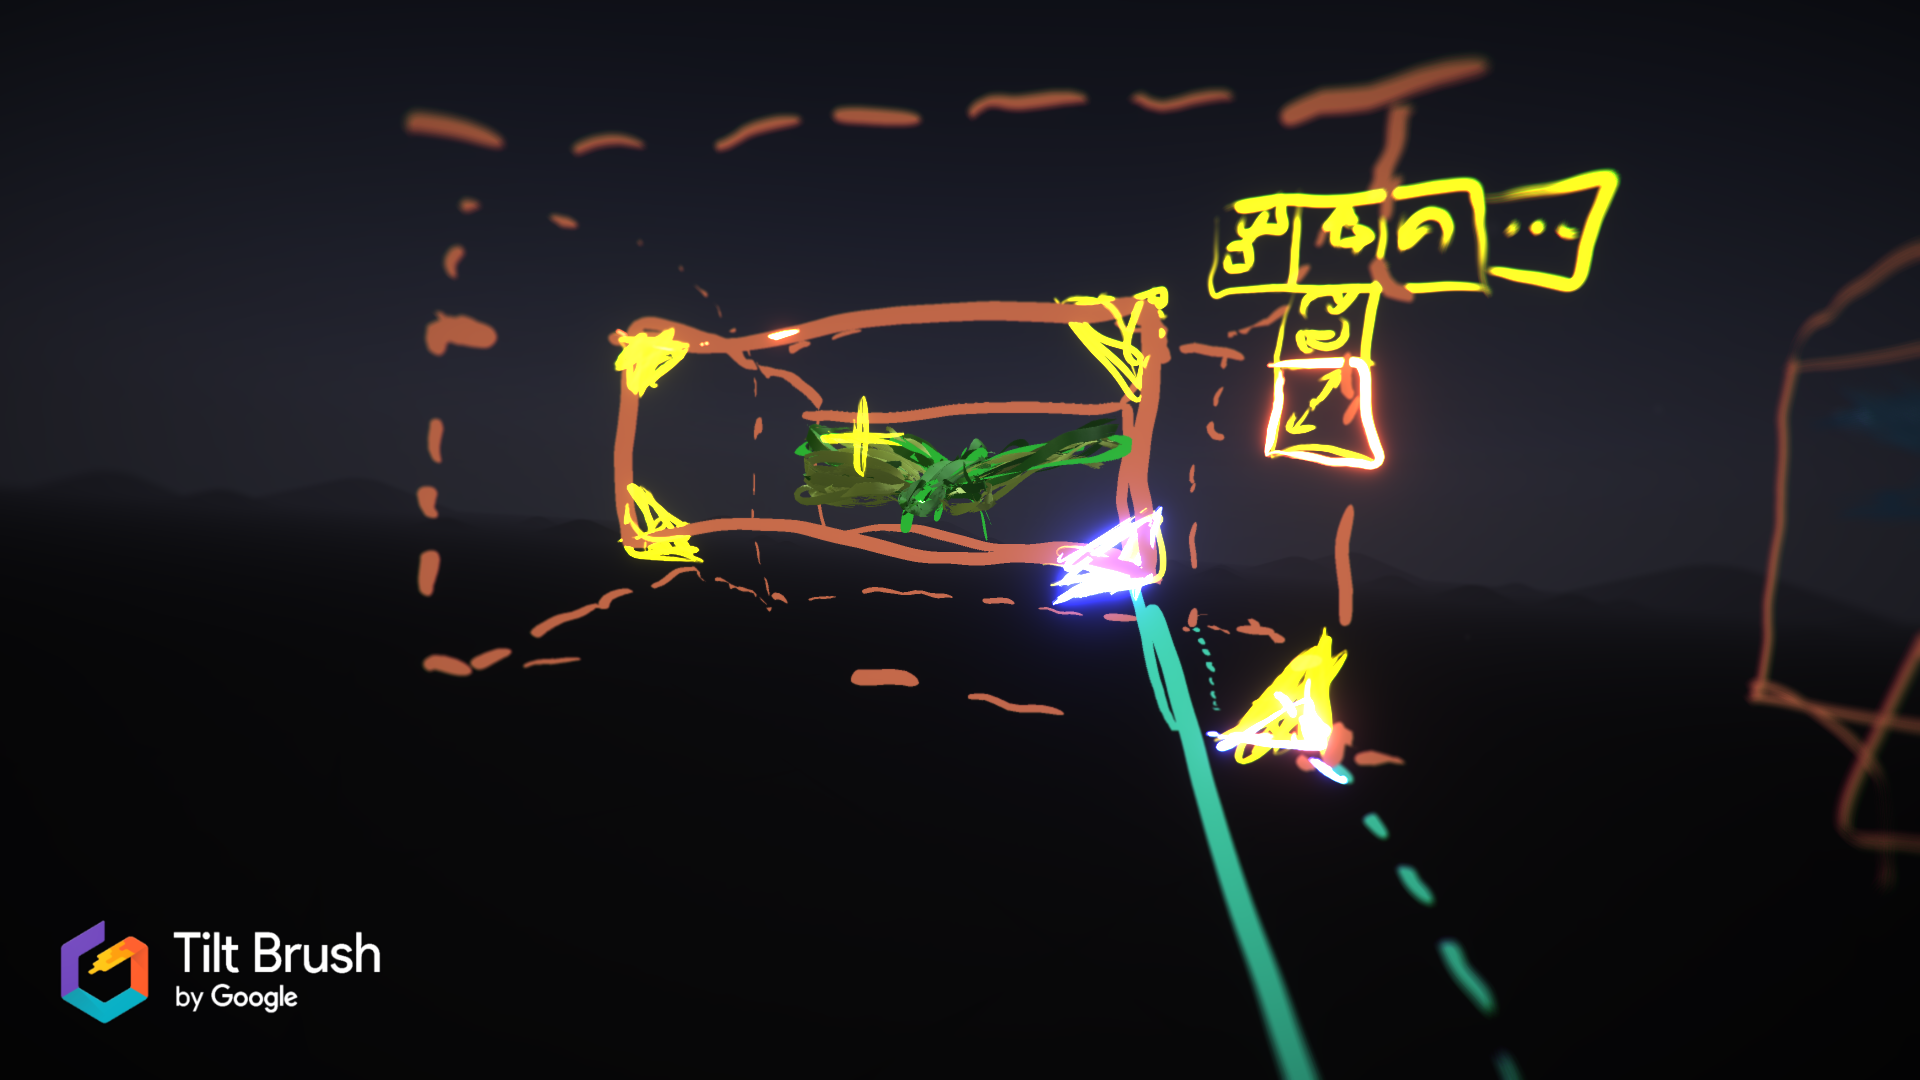
\includegraphics[width=.8\linewidth]{lo-fi/scalescenario3.PNG}
  \caption{A scale scenario where bottom right corner of a boundingbox is moved}
  \label{fig:lofi:scale3}
\end{subfigure}%
\begin{subfigure}{.5\textwidth}
  \centering
  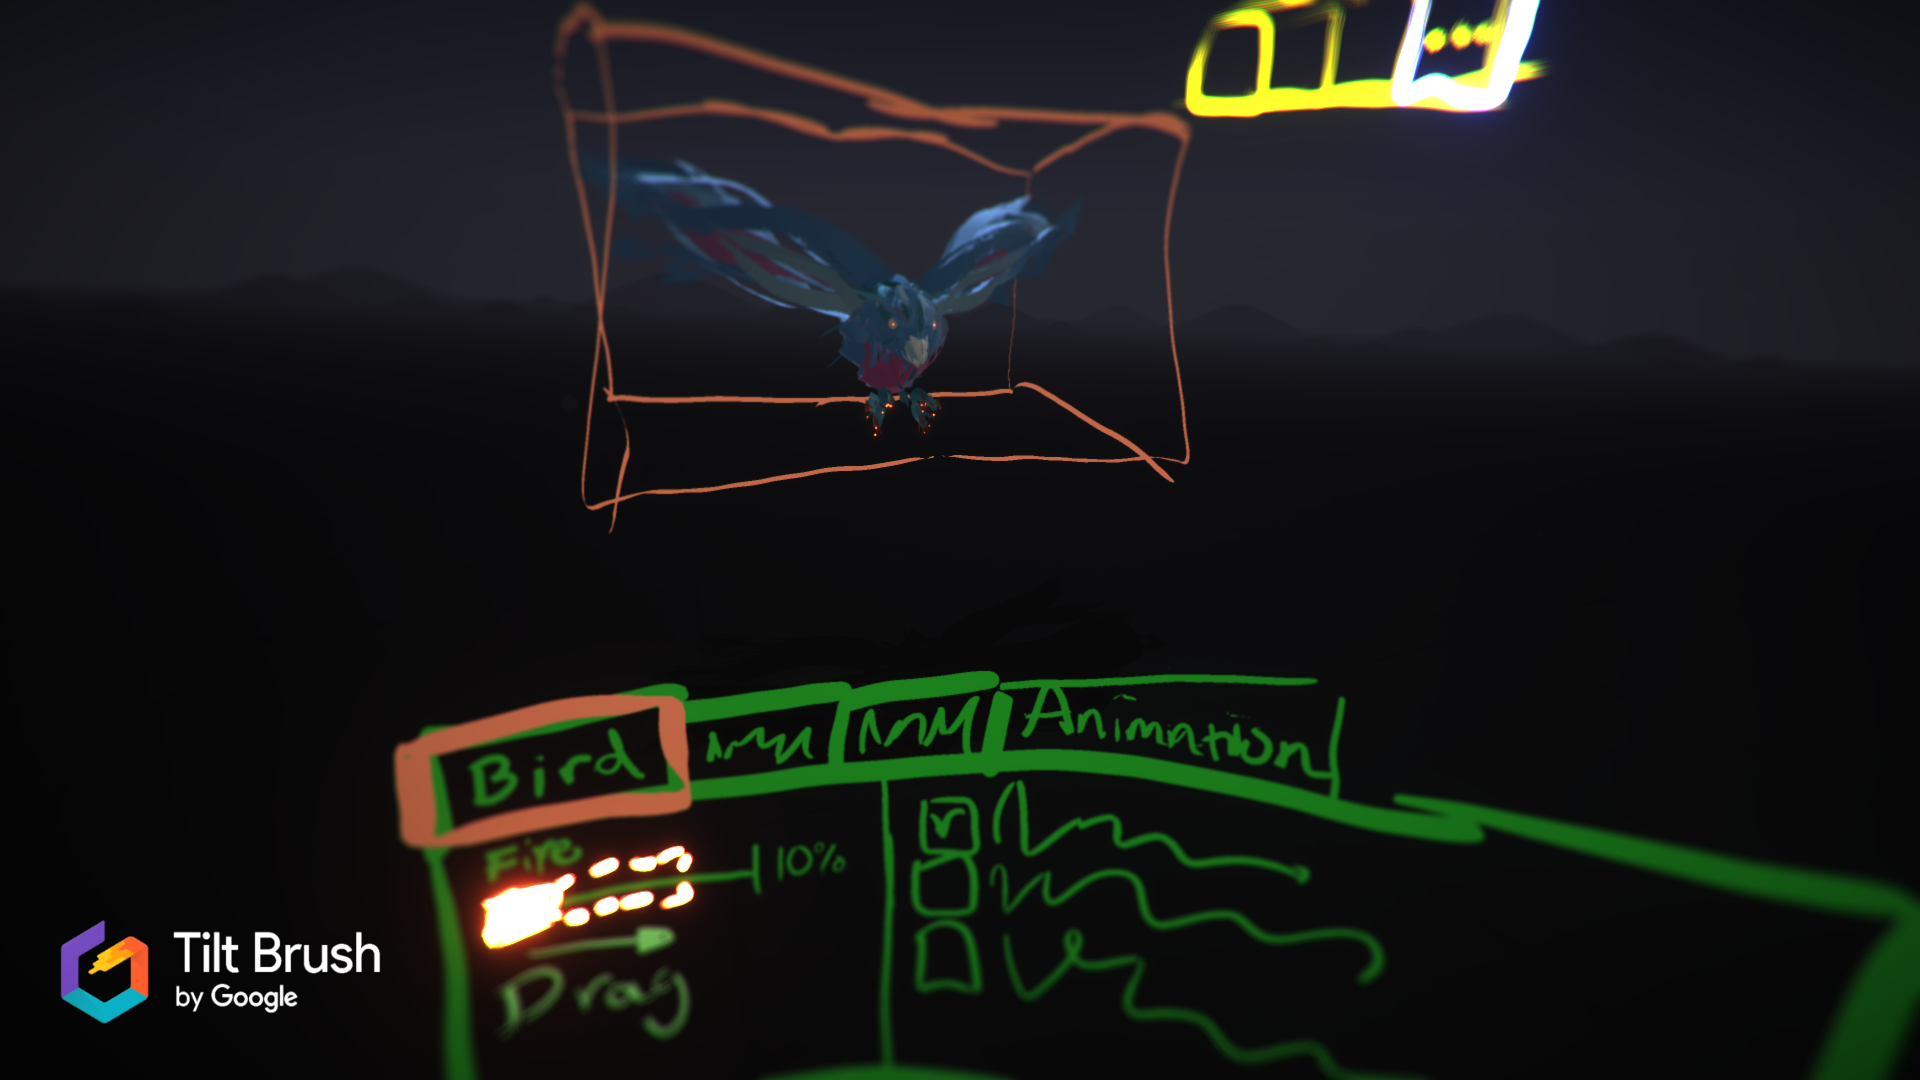
\includegraphics[width=.8\linewidth]{lo-fi/birdmenu2.PNG}
  \caption{Accessing properties of an object}
  \label{fig:tilt:passivemenu}
\end{subfigure}
\caption{Lo-fi sketches. Created in Tilt Brush (see Section \ref{relatedwork:tiltbrush})}
\label{fig:tilt}
\end{figure}
